\documentclass[varwidth=true, border=2pt]{standalone}
\usepackage{tikz}
\usepackage{pgfplots}

\begin{document}
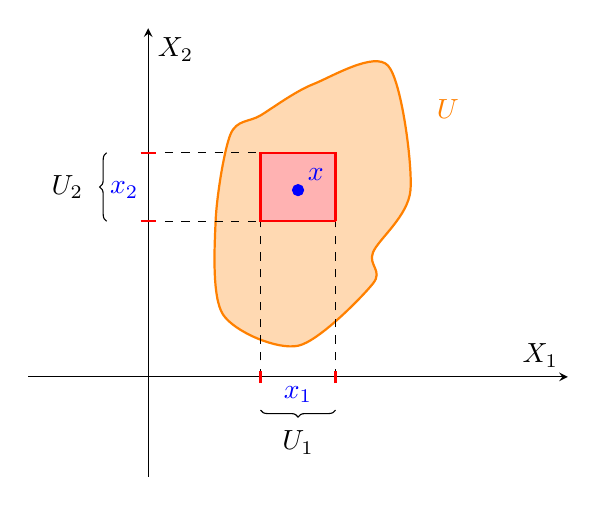
\begin{tikzpicture}
    \begin{axis}[
        axis x line=middle,
        axis y line=middle,
        %width=9cm,
        %height=4.5cm,
        xmin=-1,     % start the diagram at this x-coordinate
        xmax= 5,    % end   the diagram at this x-coordinate
        ymin=-1,     % start the diagram at this y-coordinate
        ymax= 5,   % end   the diagram at this y-coordinate
        xlabel=$X_1$,
        ylabel=$X_2$,
        ticks=none,
        enlargelimits=true,
        after end axis/.code={
            \draw [decorate,decoration={brace,mirror,raise=15pt}] (axis cs:0,3.6) -- (axis cs:0,2.5) node [midway,left=20pt] {$U_2$};
            \draw [decorate,decoration={brace,mirror,raise=12pt}] (axis cs:1.5,0) -- (axis cs:2.5,0) node [midway,below=16pt] {$U_1$};
        }]

        \addplot[mark=none, orange, smooth cycle, thick, fill=orange!30] coordinates {(1,1) (2,0.5) (3,1.5) (3,2) (3.5,3) (3.2, 5) (2.2, 4.7) (1.5, 4.2) (1.1, 3.9) (0.9, 2.5)};
        \node[orange] at (axis cs:4,4) [anchor=south] {$U$};

        % Draw help lines
        \addplot[dashed] coordinates {(1.5,0) (1.5,3.6)};
        \addplot[dashed] coordinates {(2.5,0) (2.5,3.6)};
        \addplot[dashed] coordinates {(0,2.5) (2.5,2.5)};
        \addplot[dashed] coordinates {(0,3.6) (2.5,3.6)};

        % Draw solid square
        \addplot[mark=none, red, thick, fill=red!30] coordinates {(2.5,2.5) (2.5,3.6) (1.5,3.6) (1.5,2.5) (2.5,2.5)};

        % Draw x and annotation
        \node[blue] at (axis cs:2,3) [anchor=south west] {$x$};
        \addplot[mark=*, blue] coordinates {(2,3)};

        % Draw ticks of help lines
        \addplot[mark=none, red, thick] coordinates {(1.5, -0.1) (1.5,0.1)};
        \addplot[mark=none, red, thick] coordinates {(2.5, -0.1) (2.5,0.1)};
        \addplot[mark=none, red, thick] coordinates {(-0.1, 2.5) (0.1,2.5)};
        \addplot[mark=none, red, thick] coordinates {(-0.1, 3.6) (0.1,3.6)};

        % Draw axis text
        \node[blue] at (axis cs:0,3) [anchor=east] {$x_2$};
        \node[blue] at (axis cs:2,0) [anchor=north] {$x_1$};

    \end{axis}
\end{tikzpicture}
\end{document}
